% Made up for the tikra benchmark.
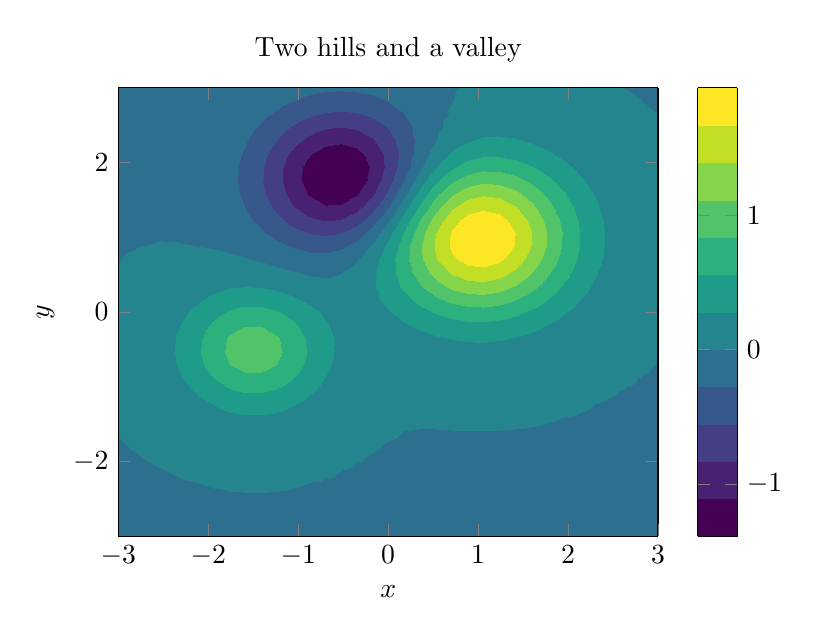
\begin{tikzpicture}
\begin{axis}[view={0}{90}, colormap/viridis, colorbar, xlabel=$x$, ylabel=$y$,
    title={Two hills and a valley}, enlargelimits=false, axis on top]
  \addplot3[contour filled={number=12}, domain=-3:3, y domain=-3:3, samples=35]
    {2*exp(-((x-1)^2+(y-1)^2)) + exp(-((x+1.5)^2+(y+0.5)^2)/0.6) - 1.5*exp(-((x+0.5)^2+(y-1.8)^2)/0.8)};
\end{axis}
\end{tikzpicture}
